% !TEX TS-program = xelatex
%
\documentclass{clseminar}

\usepackage{graphicx}
\graphicspath{{assets/}}

\usepackage{enumitem}

\usepackage{amsmath}
\usepackage{amssymb}

\usepackage{tkz-graph}
\tikzset{vertex/.style = {shape=circle,draw,minimum size=1}}
\tikzset{edge/.style = {->,> = latex'}}

\usepackage{listings}
\usepackage{color}

\definecolor{red}{RGB}{200,50,0}
\definecolor{green}{RGB}{0,150,60}

\lstdefinelanguage{mCRL2}{
  basicstyle=\ttfamily,
  sensitive = true,
  keywords={act, proc, init},
  otherkeywords={+, .},
  keywordstyle=\color{green},
  comment=[l]{\%},
  commentstyle=\color[rgb]{0.6,0.6,0.6}\itshape,
}



\usepackage[english]{babel}
\usepackage{parskip}

\usepackage{forest}

\usepackage[T1]{fontenc}
\usepackage[sorting = none]{biblatex}
\addbibresource{references.bib}

\usepackage{caption}
\usepackage{subcaption}

\title{Process Calculi for Concurrency}
\author{Markus Reiter and Michael Kaltschmid}
\supervisor{Vincent van Oostrom}

\begin{document}
  \abstract{
    This report provides a brief overview of process calculi and showcases the \textit{mCRL2} toolset. In particular we will focus on \textit{ACP} and \textit{$\mu$-Calculus}, since \textit{mCRL2} is based on both of them. At the end we provide a short introduction on how to use some of the tools provided by \textit{mCRL2}.
  }
  \maketitle
  \newpage
  \tableofcontents

  \section{Introduction}
  This report is about \textit{mCRL2}, a modern toolset for process specification and model checking. We will discuss \textit{mCRL2} itself and the concepts it is based upon.

  \subsection{What is a Process Calculus?}

  A process calculus is an approach for formally modelling concurrent systems. Furthermore it is a tool for high-level description of interactions, communication and synchronization between processes. It also provides algebraic laws to allow analyzing and transforming process descriptions and permits formal reasoning about equivalences between processes (e.g. using bisimulation). \cite{process_calculus_wiki}

  \subsection{Focus}

  There are various forms of process calculi like \textit{ACP}, \textit{CCS}, \textit{CSP}, \textit{Join-Calculus}, \textit{PEPA} or \textit{$\pi$-Calculus}. However we are only going to focus on \textit{ACP} since it a core concept of \textit{mCRL2}.

  \section{Labelled Transition Systems}

  An LTS (Labelled Transition System) is a directed labelled graph and it consists of a set of states and a set of transitions labelled with actions that connect the states. Additionally it must have an initial state. It is also important to note that it will deadlock if a reachable state does not terminate and has no outgoing
  transitions. If a state has more than one outgoing transition with the same label to different states, then it is non-deterministic.

  An LTS is a tuple $(S, A, \to,s_0>)$ where: \\

  \begin{itemize}[noitemsep]
    \item $S$ is a set of states \\
    \item $A$ is a set of actions \\
    \item $\to\ \subseteq S \times A \times S$ is a transition relation \\
    \item $s_0 \in S$ is the initial state \\
  \end{itemize}

  \begin{figure}[!ht]
    \begin{minipage}{.5\linewidth}
      \centering
      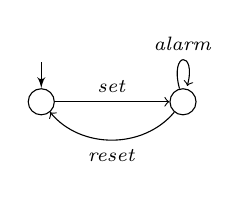
\begin{tikzpicture}[font=\sffamily\scriptsize]
  \node[vertex] (a) at (0, 0) {};
  \node[vertex] (b) at (1.8, 0) {};

  \draw[edge] (0, 0.5) to (a);
  \path[->] (a) edge  node[above] {$\mathit{set}$} (b);
  \path[->] (b) edge  [loop above] node {$\mathit{alarm}$} ();
  \path[->] (b) edge  [bend left=50] node[below] {$\mathit{reset}$} (a);
\end{tikzpicture}

      \captionof{figure}{}
      \label{fig:lts1}
    \end{minipage}
    \begin{minipage}{.5\linewidth}
      \centering
      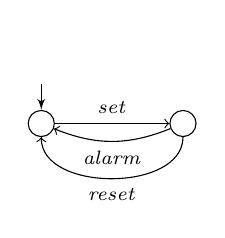
\begin{tikzpicture}[font=\sffamily\scriptsize]
  \node[vertex] (a) at (0, 0) {};
  \node[vertex] (b) at (1.8, 0) {};
  \node at (0, 1.1) {};

  \draw[edge] (0, 0.5) to (a);
  \path[->] (a) edge  node[above] {$\mathit{set}$} (b);
  \path[->] (b) edge  [bend left=22] node[below] {$\mathit{alarm}$} (a);
  \path[->] (b) edge  [bend left=90] node[below] {$\mathit{reset}$} (a);
\end{tikzpicture}

      \captionof{figure}{}
      \label{fig:lts2}
    \end{minipage}
  \end{figure}

  In \autoref{fig:lts1} and \autoref{fig:lts2} you can see examples of two LTSs for alarm clocks. The first alarm clock on the left allows for repeated alarms which can be seen by the loop on top of the alarm state. With the second alarm clock it is only possible to signal the alarm once.

  Both LTSs are deterministic since no state has more than one outgoing transition with the same label to a different state. However we can make the right LTS non-deterministic by drawing a loop on top of the alarm state as you can see in \autoref{fig:lts3}. \\

  \begin{figure}[!ht]
    \centering
    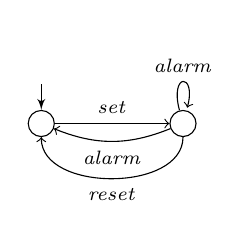
\begin{tikzpicture}[font=\sffamily\scriptsize]
  \node[vertex] (a) at (0, 0) {};
  \node[vertex] (b) at (1.8, 0) {};
  \node at (0, 1.1) {};

  \draw[edge] (0, 0.5) to (a);
  \path[->] (a) edge  node[above] {$\mathit{set}$} (b);
  \path[->] (b) edge  [bend left=22] node[below] {$\mathit{alarm}$} (a);
  \path[->] (b) edge  [loop above] node {$\mathit{alarm}$} ();
  \path[->] (b) edge  [bend left=90] node[below] {$\mathit{reset}$} (a);
\end{tikzpicture}

    \caption{}
    \label{fig:lts3}
  \end{figure}

  \subsection{Bisimulation}
  Bisimulation is a binary relation between LTSs, where LTSs behave the same way in the sense
  that one LTS simulates the other and vice versa. \cite{bisimulation_wiki} Bisimulation is not the only form of equivalence. We chose to differentiate between trace equivalence and strong bisimilarity as they are easy to show on an example.

  \begin{itemize}[noitemsep]
    \item Trace equivalence: \\
    Two LTSs are equivalent iff they can perform the same sequences of actions, starting from their initial states \\
    \item Strong bisimilarity: \\
    If one LTS can perform an action a then the other LTS must also be able to perform an action a in a way that the resulting states are again related. \\
  \end{itemize}

  \begin{figure}[!ht]
    \resizebox{\textwidth}{!}{\begin{tabular}{cc}
  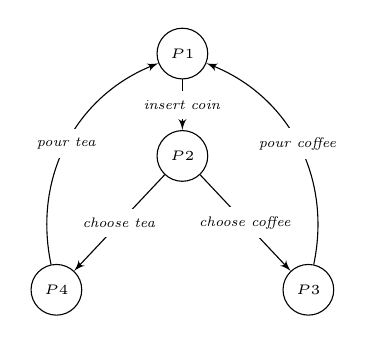
\begin{tikzpicture}[font=\sffamily\tiny]
    \node[vertex] (P1) at (1.6, 3) {$P1$};
    \node[vertex] (P2) at (1.6, 1.7) {$P2$};
    \node[vertex] (P3) at (3.2, 0) {$P3$};
    \node[vertex] (P4) at (0, 0) {$P4$};

    \path[edge] (P1) edge node[fill=white] {$\mathit{insert\ coin}$} (P2);
    \path[edge] (P2) edge node[fill=white] {$\mathit{choose\ coffee}$} (P3);
    \path[edge] (P2) edge node[fill=white] {$\mathit{choose\ tea}$} (P4);
    \path[edge] (P3) edge [bend right=40] node[fill=white] {$\mathit{pour\ coffee}$} (P1);
    \path[edge] (P4) edge [bend left=40] node[fill=white] {$\mathit{pour\ tea}$} (P1);
  \end{tikzpicture}
  &
  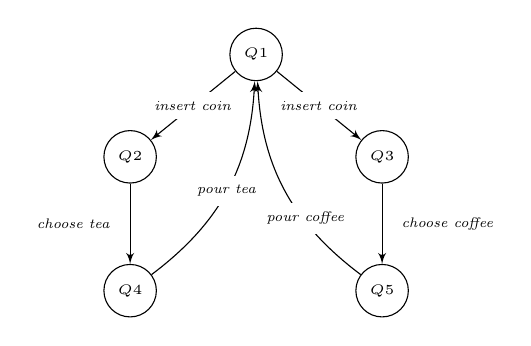
\begin{tikzpicture}[font=\sffamily\tiny]
    \node[vertex] (Q1) at (1.6, 3) {$Q1$};
    \node[vertex] (Q2) at (0, 1.7) {$Q2$};
    \node[vertex] (Q3) at (3.2, 1.7) {$Q3$};
    \node[vertex] (Q4) at (0, 0) {$Q4$};
    \node[vertex] (Q5) at (3.2, 0) {$Q5$};

    \path[edge] (Q1) edge node[fill=white] {$\mathit{insert\ coin}$} (Q2);
    \path[edge] (Q1) edge node[fill=white] {$\mathit{insert\ coin}$} (Q3);
    \path[edge] (Q2) edge node[label=left:$\mathit{choose\ tea}$] {} (Q4);
    \path[edge] (Q3) edge node[label=right:$\mathit{choose\ coffee}$] {} (Q5);
    \path[edge] (Q4) edge [bend right=25] node[fill=white] {$\mathit{pour\ tea}$} (Q1);
    \path[edge] (Q5) edge [bend left=25]  node[xshift=7.5pt, yshift=-10pt, fill=white] {$\mathit{pour\ coffee}$} (Q1);
  \end{tikzpicture}
\end{tabular}
}
    \caption{Bisimilarity of two coffee machines.}
    \label{fig:coffee_machines}
  \end{figure}

  The two coffee machines in \autoref{fig:coffee_machines} are trace equivalent but not strongly bisimilar because the resulting states are not related. As an example we can check what happens after inserting a coin. With the first coffee machine we reach state $P2$ and with the second coffee machine we reach either $Q2$ or $Q3$ depending on the choice of beverage.\\
  So the process of inserting a coin and then either getting a coffee or a tea is the same but the path and most importantly the states are different.

  \section{$\mu$-Calculus}
  As already mentioned before $\mu$-Calculus is an integral part of $mCRL2$. $\mu$-Calculus is an extension of propositional logic and therefore shares some similarities. \\
  It is used to describe and verify properties of LTSs.

  \subsection{Hennessy-Milner Logic}
  Hennessy-Milner Logic is a modal logic like LTL or CTL and for this reason we can see some relations. \\
  \begin{align*}
    \phi ::= \mathit{true}\ |\ \mathit{false}\ |\ \neg \phi\ |\ \phi \land \psi\ |\ \phi \lor \psi\ |\ \phi \to \psi\ |\ \langle a \rangle \phi \ |\ [a]\phi
  \end{align*}
  \begin{itemize}
    \item $\mathit{true}$ is true in each state of a process and $\mathit{false}$ is never true
    \item $\neg ,\ \land\ ,\ \lor$ and $\to$ as in propositional logic
    \item $\langle a \rangle \phi$ is valid whenever an $a-action$ can be performed such that $\phi$ is valid after this $a$ has been done
    \item $[a]\phi$ is valid when for every action $a$ that can be done, $\phi$ holds after doing that $a$
  \end{itemize}

  \subsection{Diamond and Box Modalities}

  Although $\langle a \rangle \phi$ - diamond modality and $[a]\phi$ - box modality look somewhat similar, yet they are very different. We can imagine the diamond modality like a $F$ in LTL and the box modality like a $G$ in LTL. \\
  In order to show the difference between the two modalities we have four simple LTSs where we take a look whether the box modality or the diamond modality of $a$ is valid.

  \begin{figure}[!ht]
   \resizebox{\textwidth}{!}{
      \newcommand{\valid}{{\color{green} valid}}
      \newcommand{\invalid}{{\color{red} invalid}}
      \renewcommand{\arraystretch}{2}
      \begin{tabular}{l c c c c}


        &

        \subcaptionbox{\label{fig:lts_a}}{
          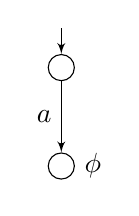
\begin{tikzpicture}
            \node[vertex] (a) at (0, 1.25) {};
            \node[vertex] [label=right:{$\phi$}] (b) at (0, 0) {};

            \draw[edge] (0, 1.75) to (a);
            \draw[edge] (a) to node [left] {$a$} (b);
          \end{tikzpicture}
        }

        &

        \subcaptionbox{\label{fig:lts_b}}{
          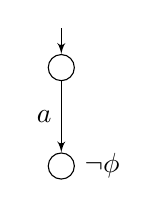
\begin{tikzpicture}
            \node[vertex] (a) at (0, 1.25) {};
            \node[vertex] [label=right:{$\neg\phi$}] (b) at (0, 0) {};

            \draw[edge] (0, 1.75) to (a);
            \draw[edge] (a) to node [left] {$a$} (b);
          \end{tikzpicture}
        }

        &

        \subcaptionbox{\label{fig:lts_c}}{
          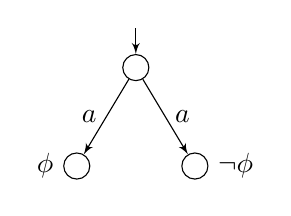
\begin{tikzpicture}
            \node[vertex] (a) at (0.75, 1.25) {};
            \node[vertex] [label=left:{$\phi$}] (b) at (0, 0) {};
            \node[vertex] [label=right:{$\neg\phi$}] (c) at (1.5, 0) {};

            \draw[edge] (.75, 1.75) to (a);
            \draw[edge] (a) to node [left] {$a$} (b);
            \draw[edge] (a) to node [right] {$a$} (c);
          \end{tikzpicture}
        }

        &

        \subcaptionbox{\label{fig:lts_d}}{
          \begin{tikzpicture}
            \node[vertex] (a) at (0, 1.25) {};
            \node at (0, -0.175) {};

            \draw[edge] (0, 1.75) to (a);
          \end{tikzpicture}
        }

        \\

        $\langle{}a\rangle{}\phi$ & \valid & \invalid & \valid & \invalid \\

        $[a]\phi$                 & \valid & \invalid & \invalid &  \valid \\
      \end{tabular}
    }
    \caption{Four LTSs.}
    \label{fig:modalities}
  \end{figure}

  In the first LTS (\autoref{fig:lts_a}) a $a$ action is possible to a state where $\phi$ holds and therefore both $\langle{}a\rangle{}\phi$ and $[a]\phi$ hold in the initial state. \\
  In the second LTS (\autoref{fig:lts_b}) there is no $a$ action to a state where $\phi$ holds and for that reason neither $\langle{}a\rangle{}\phi$ nor $[a]\phi$ hold in the initial state. \\
  In the third LTS (\autoref{fig:lts_c}) there is an $a$ action to a state where $\phi$ holds and an $a$ action to a state where $\phi$ does not hold and therefore $\langle{}a\rangle{}\phi$ is valid since there is at least one $a$ action that leads to a valid $\phi$. $[a]\phi$ is invalid because not every $a$ action leads to $\phi$. \\
  In the fourth LTS (\autoref{fig:lts_d}) there is no $a$ action at all and for that reason $\langle{}a\rangle{}\phi$ is not valid, because there needs to be an $a$ action that can be performed. However $[a]\phi$ is valid, since there is no action that can be done.

  \subsection{Regular Formulae}

  In many cases we'd like to allow for more than one single action in a modality and in this case Regular formulas are useful. \\
  An example would be that after two or more arbitrary actions, a specific action must happen or after two receive actions, a send action must follow. \\
  Regular formulas are based on Action formulas. An Action formula is a set of multi-actions, which is as follows:

  \pagebreak
  \begin{align*}
    \mathit{af} ::= \alpha\ |\ \mathit{true}\ |\ \mathit{false}\ |\ \overline{\mathit{af}}\ |\ \mathit{af}\ \cap\ \mathit{af}\ |\ \mathit{af}\ \cup\ \mathit{af}
  \end{align*}

  \begin{itemize}
    \item $\alpha$ represents the set with exactly the multi-action $\alpha$.
    \item $\mathit{true}$ is the set of all multi-actions.
    \item $\mathit{false}$ is the empty set.
    \item $\overline{\mathit{af}}$ denotes the complement of the set $\mathit{af}$.
    \item $\cup$ and $\cap$ denote union and intersection, respectively.
  \end{itemize}

  The modal formula $\langle true \rangle \langle a \rangle true$ expresses that an arbitrary action followed by an action a can be performed. \\
  The formula $[true]false$ expresses that no action can be done.

  $\mathit{af}$ being a set of multi-actions, modalities with action formulae are defined like this:

  \begin{align*}
    \langle{\mathit{af}}\rangle\phi = \bigvee_{\alpha \in \mathit{af}} \langle\alpha\rangle\phi
    \qquad\qquad
    [\mathit{af}]\phi = \bigwedge_{\alpha \in \mathit{af}} [\alpha]\phi
  \end{align*}

  As an example we can look at $\langle\overline{a}\rangle\langle{b \cup c}\rangle\mathit{true}$, which means that an action other than $a$ can be done, followed by either $b$ or $c$ \\
  $[\overline{a}]\mathit{false}$ says that only an $a$ action is allowed. \\

  Regular formulae extend action formulae by allowing sequences of actions in modalities.

  \begin{align*}
    R ::= \epsilon\ |\ \mathit{af}\ |\ R\cdot{R}\ |\ R+R\ |\ R^*\ |\ R^+
  \end{align*}

  \begin{itemize}
    \item $\epsilon$ is the empty sequence of actions.
    \item $R_1\cdot{R_2}$ represents the concatenation of $R_1$ and $R_2$.
    \item $R_1+R_2$ denotes the union of  $R_1$ and $R_2$.
    \item $R^*$ denotes zero ore more repetitions.
    \item $R^+$ denotes one ore more repetitions.
  \end{itemize}

  Since $R_1\cdot{R_2}$ denotes the concatenation of $R_1$ and $R_2$, we can write $\langle a \cdot b \cdot c \rangle true$ instead of $\langle a \rangle \langle b \rangle \langle c \rangle true$ true. Both express that the sequence of actions a, b and c can be performed. \\
  In contrast to that $[a\cdot{b} + c\cdot{d}]\mathit{false}$ means that neither the sequence $a\cdot{b}$ nor $c\cdot{d}$ is possible. \\
  Also $[a^+]\phi$ says that $\phi$ must hold in any state reachable by one or more $a$ actions. \\
  Furthermore $[\epsilon]\phi = \langle \epsilon \rangle \phi = \phi$ therefore we can always perform no action to stay in the same state. \\

  Two other commonly used formulae are the \textit{always} and \textit{eventually} modalities.\\

  \begin{align*}
    \square\phi = [\mathit{true}^*]\phi \qquad\qquad    \diamond\phi = \langle\mathit{true}^*\rangle\phi
  \end{align*}

  where $\square\phi$ means that $\phi$ holds in all reachable states and $\diamond\phi$ says that there is a sequence of actions after which $\phi$ holds. \\

  \subsection{Safety and Liveness Properties}

  The \textit{always} and \textit{eventually} modalities are further referred as Safety and Liveness properties.

  \subsubsection{Safety Property}

  \begin{align*}
    \square\phi \text{ says that something bad will never happen.}
  \end{align*}

  It is best to show this with an example. The following is a program with a critical region and two actions, enter and leave.

  \begin{align*}
    [\mathit{true}^*\cdot \mathit{enter} \cdot \overline{\mathit{leave}}^* \cdot \mathit{enter}]\mathit{false}
  \end{align*}

  In this example it is impossible to enter twice in a row. There has to be a leave action in
  between two enter actions.

  \pagebreak
  \subsubsection{Liveness Property}

  \begin{align*}
    \diamond\phi \text{ means that Something good will happen.}
  \end{align*}

  In order to demonstrate the liveness property we have a program that sends and receives messages.

  \begin{align*}
    [\mathit{true}^*\cdot \mathit{send}]\langle \mathit{true}^* \cdot \mathit{receive} \rangle \mathit{true}
  \end{align*}

  Every time a message is sent, it can eventually be received.

  \subsection{Fixed Point Modalities}

  By extending the Hennessy-Milner logic with fixed points we have:

  \begin{align*}
    \mathit{af} ::= \alpha\ |\ \mathit{true}\ |\ \mathit{false}\ |\ \neg \phi\ |\ \phi \land \psi\ |\ \phi \lor \psi\ |\ \phi \to \psi\ |\ \langle a \rangle \phi \ |\ [a]\phi\ |\ \color{green} \mu X. \phi \ |\ \nu X. \phi \ |\ X.
  \end{align*}

  \begin{itemize}
    \item $X$ is a set of states
    \item $\mu X. \phi$ is the minimal fixed point
    \item $\nu X. \phi$ is the maximal fixed point
    \item minimal and maximal fixed point operators are each other's duals
  \end{itemize}
  \begin{tabular}{cc}
    \begin{minipage}{.47\linewidth}
      \begin{align*}
        \neg \nu X. \phi = \mu X. \neg \phi
      \end{align*}
    \end{minipage}
    \begin{minipage}{.47\linewidth}
      \begin{align*}
        \neg \mu X. \phi = \nu X. \neg \phi
      \end{align*}
    \end{minipage}
  \end{tabular}

  To make us more familiar with the concept of fixed points and especially with the difference between the minimal fixed point and the maximal fixed point, we have an example with a simple LTS with exactly one state and a loop with an action $a$. \\

  \begin{center}
    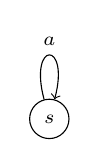
\begin{tikzpicture}[font=\sffamily\scriptsize]
      \node[vertex] (S) at (0, 0) {$s$};
      \path[->, every loop/.style={looseness=15}] (S) edge  [loop above] node {$a$} ();
    \end{tikzpicture}
  \end{center}

  \begin{example}
    The first question is if $\mu X. \langle a \rangle X$ and $\nu X. \langle a \rangle X$ hold for the state $s$. \\
    The states in question are the empty set $X = \emptyset$ and the set of all states $X = \{s\}$. \\
    $X = \emptyset$ is the same as $X = \langle a \rangle X$, which can be further reduced to $\mathit{false} = \langle a \rangle \mathit{false}$, which we can see is valid. \\
    Therefore $\mu X. \langle a \rangle X$ - minimal fixed point is valid for all states in the empty set but not in $s$ and $\nu X. \langle a \rangle X$ - maximal fixed point is valid for all states in the largest set $\{s\}$.
  \end{example}

  \section{ACP}

  ACP is the Algebra of Communicating Processes and is used to describe parallel and concurrent processes.

  In ACP, a process is defined \cite{acp_wiki} as follows:

  \begin{align*}
    P ::= a\ |\ \delta\ |\ \tau\ |\ P + P\ |\ P \cdot P\ |\ (P || P)\ |\ (P |\lfloor P)\ |\ (P | P)\ |\ \tau_I(P)
  \end{align*}

  Here, $a$ represents an atomic action, $\delta$ is the deadlock action \\ and $\tau$ is the silent action.

  $a + b$ means either $a$ or $b$ (\textit{alternative operator}), $a \cdot b$ means $a$ followed by $b$ (\textit{sequencing operator}).

  $|\lfloor$ is the left-merge operator, it is the generalized version of $||$ (\textit{merge operator}) and denotes concurrency.
  \\
  \begin{example}
    $(a \cdot b) |\lfloor (c \cdot d)$ ensures that the left branch is started first, in this case that $a$ occurs first, so only the sequences $abcd$, $acdb$ and $acbd$ are possible.

    $(a \cdot b) || (c \cdot d)$ is therefore actually an alternative between $(a \cdot b) |\lfloor (c \cdot d)$ and $(c \cdot d) |\lfloor (a \cdot b)$.
  \end{example}

  $|$ is the called the communications operator and is used do pass data between actions.
  \\
  \begin{example}
     $r(d) | w(d)$ means that the value $d$ is communicated from action $w$ from the right side to $r$ on the left side.
  \end{example}

  $\tau_I$ is the abstraction operator. It is used to “hide” certain actions.
  \\
  \begin{example}
    $\tau_{\{c\}}((a+b)\cdot c)$ is equal to $(a + b) \cdot \tau$, which can be reduced to $a + b$.
  \end{example}

  \section{mCRL2}

  \textbf{mCRL2} is a toolset which is used for specifying and analysing behaviour of distributed systems and protocols. We chose this tool because it uses an ACP-like syntax for its formal specification language for processes as well as $\mu$-Calculus for model checking.

  \subsection{Process Specification}

  Let's first take a look at the \textbf{mCRL2} syntax for specifying processes. Usually, a process specification file will have a file name of the form \texttt{*.mcrl2}.

  \begin{figure}[!ht]
    \begin{lstlisting}[language=mCRL2]
act a, b, c, d, e;

proc P = a . b . c;
     Q = d + e;
     R = (a + b) . c . d . e;

init P;
    \end{lstlisting}
    \caption{The \textbf{mCRL2} process specification syntax.}
    \label{fig:mcrl2_syntax}
  \end{figure}

  As you can see in the first line in \autoref{fig:mcrl2_syntax}, we specify all available actions using the \texttt{act} keyword. This relates to atomic actions in the ACP syntax. Now that we have defined the actions, we can specify the process itself, or multiple processes, if there are more than one. We do this using the \texttt{proc} keyword, followed by the name of the process. In \autoref{fig:mcrl2_syntax} we have three processes, \texttt{P}, \texttt{Q} and \texttt{R}. We then equate every process with a combination of actions, action sequences, action alternatives. Processes themselves can also be used on the right-hand side, which is essential for recursion. In \textbf{mCRL2}, we use \texttt{.} to denote a sequence and \texttt{+} to denote an alternative. This means that process \texttt{P} is a sequence of actions \texttt{a}, \texttt{b} and \texttt{c}. Process \texttt{Q} is a choice between either action \texttt{d} or action \texttt{e}. And finally, process \texttt{R} is a choice between action \texttt{a} and \texttt{b}, followed by \texttt{c}, \texttt{d} and \texttt{e}. Note the parentheses around \texttt{a + b}, since \texttt{.} binds stronger than \texttt{+}. Finally, the \texttt{init} keyword specifies the starting process, in this case \texttt{P}.

  To demonstrate the power of ACP and $\mu$-Calculus in combination with the \textbf{mCRL2} toolset, we will now look at an implementation of the two coffee machines (\autoref{fig:coffee_machines}) in \textbf{mCRL2}.

  First, we have to define the actions for coffee machine 1.

  \begin{lstlisting}[language=mCRL2]
act insert_coin, choose_coffee, choose_tea,
                   pour_coffee,   pour_tea;
  \end{lstlisting}

  The \texttt{insert\_coin} action is self-explanatory. \texttt{choose\_coffee} and \texttt{choose\_tea} denote the actions of pressing either the button for coffee, or the button for tea. And finally, \texttt{pour\_coffee} and \texttt{pour\_tea} denote the action of dispensing either coffee or tea.

  Since coffee machine 2 is trace equivalent to coffee machine 1, it has the same actions.

  Next, we define the process for coffee machine 1.

  \begin{lstlisting}[language=mCRL2]
proc P = insert_coin . (
           choose_coffee . pour_coffee +
           choose_tea . pour_tea
         ) . P;
  \end{lstlisting}

  We start by inserting a coin (\texttt{insert\_coin}). Then, we are left with a choice between choosing coffee and pouring coffee or choosing tea and pouring tea. We see that choosing coffee or tea is tightly coupled to pouring it, since this is a choice between two sequences \texttt{(choose\_coffee . pour\_coffee)} and \texttt{(choose\_tea . pour\_tea)}. This is of course because we don't want the machine to dispense tea when in fact we chose coffee.

  The last action is \texttt{P} itself, which results in a recursion. This is because we want the machine to be reusable.

  We now define the process for coffee machine 2.

  \begin{lstlisting}[language=mCRL2]
proc Q = (
           (insert_coin . choose_coffee . pour_coffee) +
           (insert_coin . choose_tea . pour_tea)
         ) . Q;
  \end{lstlisting}

  For this machine, we specify a process named \texttt{Q}. This process starts with a choice, which is either a sequence of inserting a coin, choosing coffee and pouring coffee or inserting a coin, choosing tea and pouring tea. In comparison to the first machine, the \texttt{insert\_coin} action is now part of the choice between coffee or tea.

  Lastly, we need to specify the starting process for both machines,

  \begin{lstlisting}[language=mCRL2]
init P;
  \end{lstlisting}

  and

  \begin{lstlisting}[language=mCRL2]
init Q;
  \end{lstlisting}

  respectively.

  \subsection{Process Properties}

  Now that we have specified the processes for two coffee machines, we want to define some properties they adhere to.

  In \textbf{mCRL2}, these properties are defined in \texttt{*.mcf} (\textbf{m}odel \textbf{c}hecking \textbf{f}ormula) files and expressed by regular formulae.

  We start with a simple property: The machine does only pour coffee after coffee is chosen. For this, we use a box modality which is false if any sequence of actions that are not \texttt{choose\_coffee} is followed by \texttt{pour\_coffee}.

  \begin{lstlisting}[language=mCRL2]
[!choose_coffee* . pour_coffee]false
  \end{lstlisting}

  The \textbf{mCRL2} syntax for formulae uses \texttt{[} and \texttt{]} for box modalities.

  The second property is the counterpart to the first. The machine should only pour tea if in fact we chose tea.

  \begin{lstlisting}[language=mCRL2]
[!choose_tea* . pour_tea]false
  \end{lstlisting}

  With our third property, we want to ensure that the machine is reusable.

  \begin{lstlisting}[language=mCRL2]
[true* . (pour_tea + pour_coffee) . insert_coin]true
  \end{lstlisting}

  After any valid sequence of actions (\texttt{true*}) which ends with pouring either coffee or tea (\texttt{pour\_tea + pour\_coffee}), inserting a coin is possible.

  Lastly, we define a property which guarantees that the machine does not allow choosing a beverage without payment.

  \begin{lstlisting}[language=mCRL2]
[!insert_coin* . (choose_tea + choose_coffee)]false
  \end{lstlisting}

  For that, we define that any sequence of actions which are \textit{not} \texttt{insert\_coin}, followed by choosing coffee or tea, is invalid.

  \subsection{Model Checking}

  We have now seen how to specify processes and process properties using \textbf{mCRL2}, but we have not yet used any tool provided by it.

  For model checking we need three tools, which are provided by \textbf{mCRL2} as command line utilities. First, we need \texttt{mcrl22lps} to convert our \texttt{*.mcrl2} process specification into an LPS \cite[Linear Process Specifications]{mcrl2doc}. An LPS is a process specification with a very simple structure, which we can then convert into a so-called PBES \cite[Parametrized Boolean Equation Systems]{mcrl2doc} using \texttt{lps2pbes}. \textbf{mCRL2} can then check wether a given formula holds by solving this set of equations. This is done with the \texttt{pbes2bool} tool.

  We will now look at a specific example using our coffee machines.

  We assume the following directory structure\footnote{You can find all files in the accompanying ZIP archive if you want to try these tools yourself.}:

  \begin{forest}
    for tree={
      font=\ttfamily,
      grow'=0,
      child anchor=west,
      parent anchor=south,
      anchor=west,
      calign=first,
      edge path={
        \noexpand\path [draw, \forestoption{edge}]
        (!u.south west) +(7.5pt,0) |- node[fill,inner sep=1.25pt] {} (.child anchor)\forestoption{edge label};
      },
      before typesetting nodes={
        if n=1
          {insert before={[,phantom]}}
          {}
      },
      fit=band,
      before computing xy={l=15pt},
    }
    [./
      [coffee\_machine\_1.mcrl2]
      [coffee\_machine\_2.mcrl2]
      [properties
        [choose\_coffee\_to\_pour\_coffee.mcf]
        [choose\_tea\_to\_pour\_tea.mcf]
        [insert\_coin\_after\_pour.mcf]
        [no\_free\_coffee.mcf]
      ]
    ]
  \end{forest}

  We want to check that coffee machine 1 never gives out free coffee.

  First, we convert our process specification into an LPS:

  \begin{lstlisting}[language=Bash]
mcrl22lps coffee_machine_1.mcrl2 coffee_machine_1.lps
  \end{lstlisting}

  Next, we convert the LPS we just created into a PBES:

  \begin{lstlisting}[language=Bash]
lps2pbes -f properties/no_free_coffee.mcf coffee_machine_1.lps properties/no_free_coffee.coffee_machine_1.pbes
  \end{lstlisting}

  Here, with the \texttt{-f} flag, we specify the formula which should be checked.

  Finally, we use \texttt{pbes2bool} to solve the PBES.

  \begin{lstlisting}[language=Bash]
pbes2bool properties/no_free_coffee.coffee_machine_1.pbes
  \end{lstlisting}

  If we additionally pass the \texttt{-v} flag, we can see the strategies used to solve the equation. Here is the output for our property:

  \begin{lstlisting}
Guessing input format: PBES in internal format
pbes2bool parameters:
  input file:            properties/no_free_coffee.coffee_machine_1.pbes
  data rewriter:         jitty
  substitution strategy: 0
  search strategy:       breadth-first
  solution strategy      lf
  erase level:           none
Loading PBES in pbes format...
Processed 1 and generated 1 boolean variables.
Generated 1 BES equations in total, generating BES
Solving a BES with 1 equations using the local fixed point algorithm.
Solving equations of rank 0.
The solution for the initial variable of the pbes is true
true
  \end{lstlisting}

  With the appropriate flags, you can manually specify which strategies should be used. These can be found in the documentation \cite{mcrl2doc} or by using the tool's help flag (\texttt{-h}).

  In the last line of the output, we can see \texttt{true}. This boolean value represents wether the formula holds. This means that our property \texttt{no\_free\_coffee.mcf} holds for our first coffee machine \texttt{coffee\_machine\_1.mcrl2}

  \subsection{LTS}

  An LTS is a useful way of getting a visual overview of a process. The \texttt{lps2lts} command can be used to convert an LPS into an LTS.

  \begin{lstlisting}[language=Bash]
lps2lts coffee_machine_1.lps coffee_machine_1.lts
  \end{lstlisting}

  We can now view the LTS with the \texttt{ltsgraph} command:

  \begin{lstlisting}[language=Bash]
ltsgraph coffee_machine_1.lts
  \end{lstlisting}

  This opens a GUI (\autoref{fig:ltsgraph}) which allows you to interactively traverse the graph and view it in full.

  \begin{figure}[!ht]
    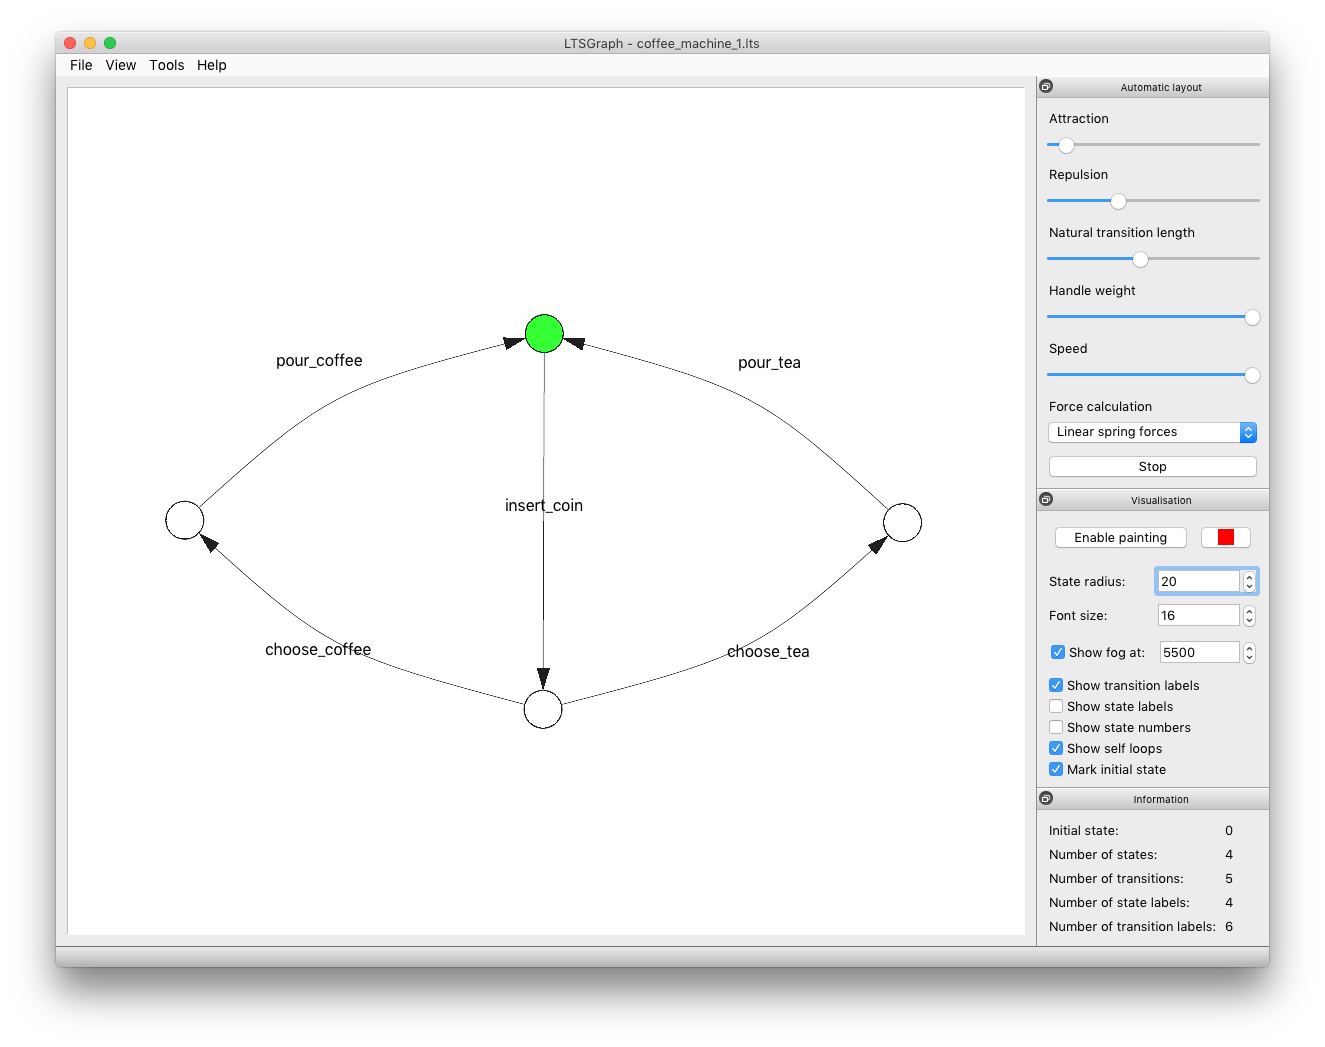
\includegraphics[width=\textwidth]{ltsgraph.png}
    \caption{\texttt{ltsgraph} window showing \texttt{coffee\_machine\_1.lts}.}
    \label{fig:ltsgraph}
  \end{figure}

  As you can see in \autoref{fig:ltsgraph}, the green circle represents the starting state. In the \textit{Automatic Layout} section, you can click \textit{start} to automatically lay out the graph, which usually makes it much more readable. You can then drag the state circles around and by right-clicking them, you can fix their positions, so that they are not affected by the automatic layout anymore. One additional feature is \textit{Exploration Mode}. You can access it from the \textit{Tools} menu. In this mode, you can step from one state, beginning in the starting state, to all states that are reachable from it.

  \subsection{Bisimilarity}

  The last tool we want to demonstrate is \texttt{ltscompare}, which as the name implies is used to compare two LTSs.

  We already know that our two coffee machines are trace equivalent, but not bisimilar. We now want to check this with \texttt{ltscompare}.

  First, we need to generate the LTSs for our two coffee machines.

  \begin{lstlisting}[language=Bash]
mcrl22lps coffee_machine_1.mcrl2 coffee_machine_1.lps
mcrl22lps coffee_machine_2.mcrl2 coffee_machine_2.lps

lps2lts coffee_machine_1.lps coffee_machine_1.lts
lps2lts coffee_machine_2.lps coffee_machine_2.lts
  \end{lstlisting}

  Next, we run \texttt{ltscompare} and pass \texttt{-{}-equivalence} to specify which equivalence should be used, in our case \texttt{bisim}.

  \begin{lstlisting}[language=Bash]
ltscompare --equivalence=bisim coffee_machine_1.lts coffee_machine_2.lts
  \end{lstlisting}

  Again, all available equivalences can be seen in the tool's help page (\texttt{-h} flag) or in the \texttt{mCRL2} documentation \cite{mcrl2doc}.

  From the command, we get the following output:

  \begin{lstlisting}
LTSs are not equal (strong bisimilarity using the O(m log n) algorithm [Groote/Jansen/Keiren/Wijs 2017])
  \end{lstlisting}

  So in fact, the two LTSs are not bisimilar. We know, however, that they are trace equivalent. We can verify this using the \texttt{trace} option for \texttt{-{}-equivalence}.

  \begin{lstlisting}[language=Bash]
ltscompare --equivalence=trace coffee_machine_1.lts coffee_machine_2.lts
  \end{lstlisting}

  And indeed, we get the following output:

  \begin{lstlisting}
LTSs are equal (strong trace equivalence)
  \end{lstlisting}

  \section{Conclusion}

  TODO

  \backmatter

  \phantomsection{\addcontentsline{toc}{section}{\bibname}}
  \printbibliography
\end{document}
